\section{System Structure}

\label{sec:system_structure_appendix}

In this section a brief overview of the expected system architecture that will be developed in work package WP1 will be given. This structure is shown in figure \ref{fig:system_structure}.

\begin{figure}[h!]
  \centering
    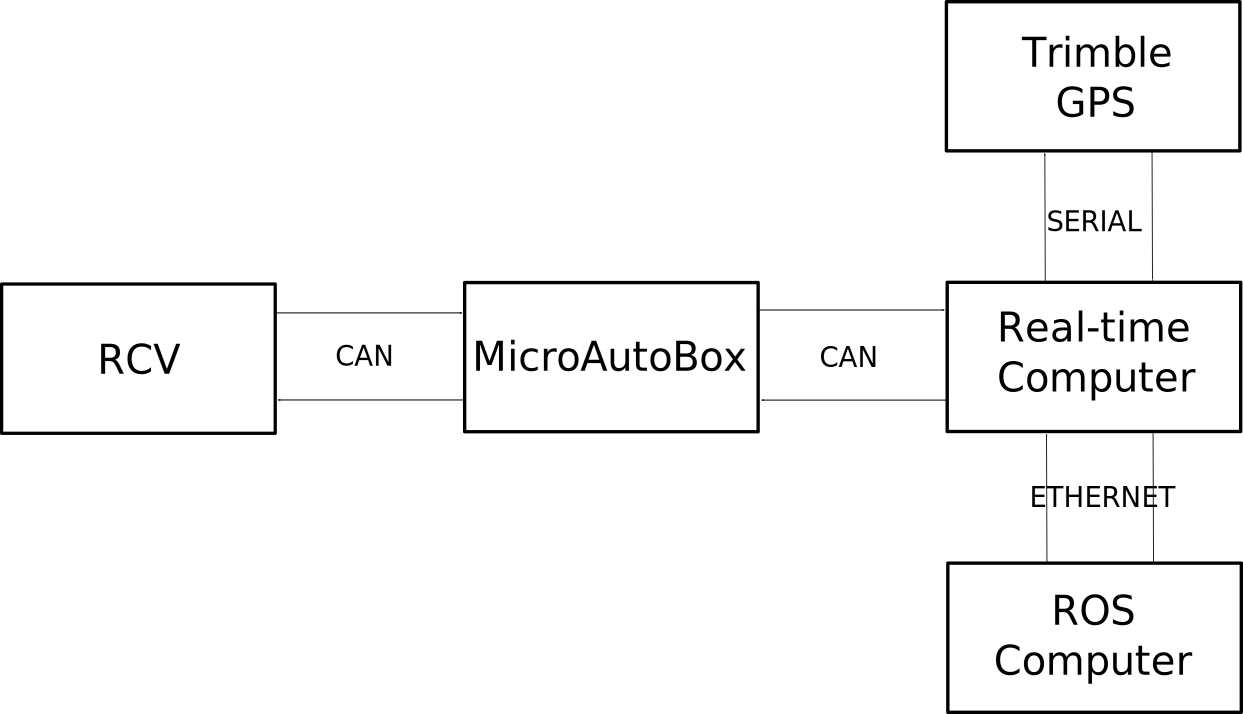
\includegraphics[width=0.8\textwidth]{SystemStructureWithCommunicationProtocols}
    \caption{Representation of the system structure to be developed in WP1 \label{fig:system_structure} }
\end{figure}

The components and their functionalities are as follows.

\subsection{RCV} 

RCV is the vehicle in itself, it is composed of all the low level sensors and actuators mounted on it. The low level sensors considered are:

\begin{itemize}
\item Encoders measuring wheel rotation for each of the four wheels
\item Encoders measuring the steering angle for each of the four wheels
\item Inertial measurement unit
\end{itemize}

The GPS is left out as it is not interfaced with in the same way as the previously mentioned sensors.

\subsection{MicroAutoBox}

The MicroAutoBox (MAB) is a real-time computer that is placed on the RCV.
It is currently responsible for the low level control of the actuators existing in the vehicle, such as the steering and torque actuators. It also gathers all of the data measured in the low level sensors in the RCV.

The MAB is able to interface with a higher level controller, which can send steering angle and torque requests. Besides receiving these requests, the MAB also sends the low level sensor data to the upper level controller. These communications are done through a CAN interface.

The MAB is somewhat limited, in the sense that it has a low processing power, and that it has a very restrictive physical interface (can only be interfaced with through CAN).

\subsection{Controller Computer} 

This is a real-time computer where the high level path following control algorithm will be implemented. Contrarily to the MAB, this is a somewhat powerful computer, and with user friendly interfaces such as Ethernet.

The Controller Computer will send steering angle and torque requests to the MAB, and it will receive from it the low level sensor readings.
It will also get the GPS readings from the Trimble system, and use them for the execution of the control algorithm.

Through UDP messaging over Ethernet, the Controller Computer will interface with the ROS Computer, receiving high level path requests (in the form of UTM coordinates), and sending the low level RCV sensor readings and GPS measurements.


\subsection{Trimble GPS}

The Trimble GPS is a system which provides accurate position estimates. It will be connected to the Controller Computer through its Serial bus.

\subsection{ROS Computer}

The ROS Computer will be a NUC running a ROS interface which allows users to send path requests to the RCV (by offering a ROS service), and to get low level sensor data and GPS readings from the vehicle (by publishing ROS topics).

